\documentclass[tikz,border=8pt]{standalone}

\usepackage[T1]{fontenc}
\usepackage{lmodern}
\usetikzlibrary{arrows.meta}

\begin{document}
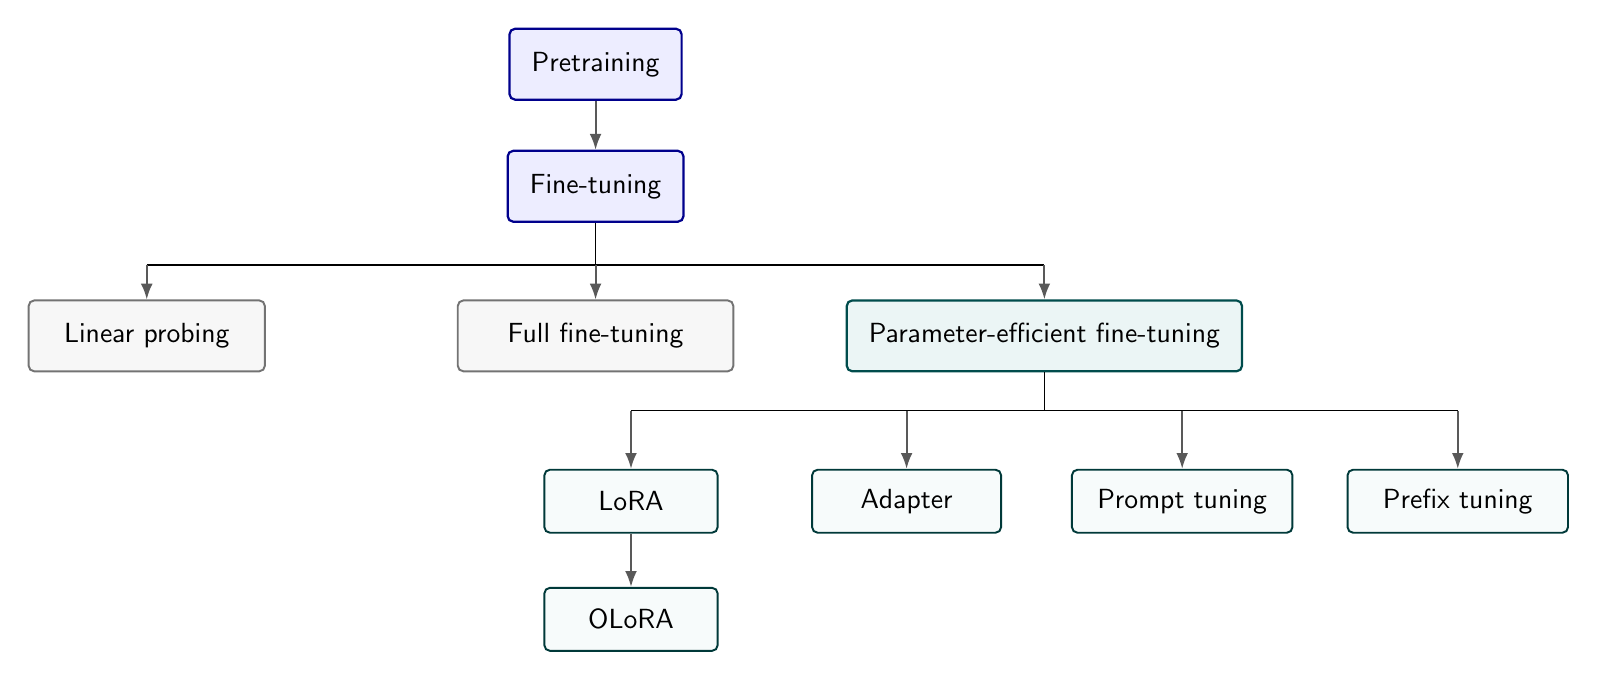
\begin{tikzpicture}[
		font=\sffamily,
		phase/.style={
				draw=blue!55!black,
				fill=blue!7,
				rounded corners=2pt,
				line width=0.8pt,
				minimum height=9mm,
				inner xsep=8pt,
				align=center,
			},
		method/.style={
				draw=black!55,
				fill=black!3,
				rounded corners=2pt,
				line width=0.7pt,
				minimum height=9mm,
				inner xsep=8pt,
				align=center,
			},
		peft/.style={
				draw=teal!60!black,
				fill=teal!8,
				rounded corners=2pt,
				line width=0.8pt,
				minimum height=9mm,
				inner xsep=8pt,
				align=center,
			},
		variant/.style={
				draw=teal!45!black,
				fill=teal!3,
				rounded corners=2pt,
				line width=0.7pt,
				minimum height=8mm,
				inner xsep=8pt,
				align=center,
			},
		connector/.style={
				draw=black!65,
				line width=0.7pt,
					-{Latex[length=2mm]},
			},
	]

	% The overall training stages.
	\node[phase] (pretraining) at (0,0) {Pretraining};
	\node[phase] (finetuning) at (0,-1.55) {Fine-tuning};
	\draw[connector] (pretraining.south) -- (finetuning.north);

	% Fine-tuning approaches.
	\node[method, minimum width=3.0cm] (linear) at (-5.7,-3.45) {Linear probing};
	\node[method, minimum width=3.5cm] (full) at (0,-3.45) {Full fine-tuning};
	\node[peft, minimum width=4.0cm] (peft) at (5.7,-3.45)
	{Parameter-efficient fine-tuning};

	\coordinate (approach-junction) at (0,-2.55);
	\draw (finetuning.south) -- (approach-junction);
	\draw (-5.7,-2.55) -- (5.7,-2.55);
	\draw[connector] (-5.7,-2.55) -- (linear.north);
	\draw[connector] (0,-2.55) -- (full.north);
	\draw[connector] (5.7,-2.55) -- (peft.north);

	% Parameter-efficient fine-tuning methods.
	\node[variant, minimum width=2.2cm] (lora) at (0.45,-5.55) {LoRA};
	\node[variant, minimum width=2.4cm] (adapter) at (3.95,-5.55) {Adapter};
	\node[variant, minimum width=2.8cm] (prompt) at (7.45,-5.55)
	{Prompt tuning};
	\node[variant, minimum width=2.8cm] (prefix) at (10.95,-5.55)
	{Prefix tuning};

	\coordinate (peft-junction) at (5.7,-4.4);
	\draw (peft.south) -- (peft-junction);
	\draw (0.45,-4.4) -- (10.95,-4.4);
	\draw[connector] (0.45,-4.4) -- (lora.north);
	\draw[connector] (3.95,-4.4) -- (adapter.north);
	\draw[connector] (7.45,-4.4) -- (prompt.north);
	\draw[connector] (10.95,-4.4) -- (prefix.north);

	% OLoRA is shown as a LoRA variant.
	\node[variant, minimum width=2.2cm] (olora) at (0.45,-7.05) {OLoRA};
	\draw[connector] (lora.south) -- (olora.north);
\end{tikzpicture}
\end{document}
